\bchapter{Differentation}

The derivative of a function of real variable is one of the major concepts of calculus. It measures the
sensitivity to change of the function value with respect to a change in its argument. For this reason, the
derivative is a powerful tool not only in maths and physics, but in other areas such as economics and, of
course, computer science.

\section{Definition of derivative and differentiable functions}

\begin{defi}[Derivative]\label{def:derivative}
    Let $\appl{f}{\dom{f}\subset \R}{\R}$ be a continuous function. Then, $f$ is differentiable at a point
    $x_0\in \dom{f}\iff$ there exists the finite limit of the difference quotient $\Delta f\left( x \right)
        / \Delta x$.
    \begin{equation}
        f'\left( x_0 \right) = \dv{x} f\left( x_0 \right) \bydef \lim_{x\to x_0} \frac{\Delta f\left( x \right) }{\Delta x} = \lim_{x\to x_0}\frac{f\left( x \right) - f\left( x_0 \right) }{x - x_0}.
    \end{equation}
\end{defi}

\hide{
Also, $f$ is differentiable in $x_0\in A \iff$ there exists a function $R:\left( x_0 - \delta, x_0 + \delta
        \right) $ and $m\in\R$ such that
        \begin{equation}
            f\left( x \right) = \underbrace{f\left( x_0 \right) + m\left( x - x_0 \right)}_{\textrm{tangent in $x_0$, $m = f'\left( x_0 \right) $}} + R\left( x \right),\quad\quad R\left( x \right)\overset{x\to x_0}{\longrightarrow} 0.
        \end{equation}
}

\noindent The difference quotient on \eref{def:derivative} is also usually written as the
following expression,
\begin{equation}
    \dv{x} f\left( x_0 \right) = \lim_{h\to 0}\frac{f\left( x_0 + h \right) - f\left( x \right) }{h},
\end{equation}
known as Newton's difference quotient.

The full derivation for the derivative can be found on mostly any calculus book or even \href{https://en.wikipedia.org/wiki/Derivative}{Wikipedia}.

\begin{prop}
    A function $f$ is differentiable within an interval $I\subseteq\R$ if it is differentiable in all points
    $x_0\in I$.
\end{prop}

\begin{notation}
    $C^1\left( I \right)$ is the space of the differentiable functions in the interval $I$.
\end{notation}

\hide{
\begin{defi}[Differential]
    We denote the differential of $f$ in a point $x_0$ by $\dd{f\left( x_0 \right)} = m\dd{x}$.
\end{defi}
}

\begin{defi}[Derivative function]
    The derivative function of $f$, or simply the derivative of $f$, is the function obtained by differentiating
    $f$ in every point $x_0\in I$.
\end{defi}

\begin{remark}
    This definition of derivative is only true when working with just one single variable.
\end{remark}

\hide{
\begin{prop}
    If $f$ is a function differentiable in the point $x_0\in\dom{f}\implies f$ is continuous in $x_0\in\dom{f}$.
\end{prop}
}

\begin{prop}
    Let $\appl{f}{I}{\R}$. If $f$ is differentiable at a point $x_0\in I$, then $f$ is continuous at $x_0$.
\end{prop}

\begin{proof}
    If $f$ is differentiable at $x_0$ we can write
    \begin{equation}
        \lim_{x\to x_0} \left( f\left( x \right) - f\left( x_0 \right) \right) = \lim_{x\to x_0}\frac{f\left( x \right)  - f\left( x_0 \right) }{x - x_0} \left( x - x_0 \right) = f'\left( x_0 \right) \cdot 0 = 0,
    \end{equation}
    in other words, $f$ is continuous in $x_0$.
\end{proof}

\noindent In general, the converse of this theorem is not true.

\noindent Since a derivative is actually a limit, it \textit{inherits} its properties.

\begin{prop}
    Let $\appl{f, g}{\R}{\R}$ be two differentiable functions at a point $x\in\dom{f}\cap\dom{g} = I$.
    \begin{itemize}[itemsep = -2pt]
        \item The derivative is a linear operation, in other words, $\forall\lambda, \mu\in\R$,
            \begin{equation}
                \brackets{\lambda f\left( x \right) \pm \mu g\left( x \right) }' = \lambda f'\left( x \right) +
                \mu g'\left( x \right), \quad \forall x\in I.
            \end{equation}
        \item The derivative of a product of functions is given by \textbf{Leibniz's rule},
            \begin{equation}
                \brackets{f\left( x \right)g\left( x \right) }' = f'\left( x \right) g\left( x \right) +
                f\left( x \right) g'\left( x \right),\quad \forall x\in I.
            \end{equation}
        \item The derivative of a composite function is given by the \textbf{chain rule},
            \begin{equation}
                \brackets{g\left( f\left( x \right)  \right) }' = g'\left( f\left( x \right)  \right) f'\left( x \right),\quad\forall x\in I.
            \end{equation}
    \end{itemize}
\end{prop}

\noindent The derivative of a quotient derives from putting the chain rule and Leibniz's rule:
\begin{equation}
    \dv{x} \frac{f\left( x \right) }{g\left( x \right) } = \frac{f'\left( x \right) g\left( x \right) -
    f\left( x \right) g'\left( x \right) }{\brackets{g\left( x \right) }^2}.
\end{equation}
At the end of these notes there is a differentiation table which puts together all the rules for differentiating analytic functions and common expressions, such as the multiplicative inverse of a function. Their
corresponding proofs can be found on most of the available calculus books or even Wikipedia.

\begin{prop}\label{prop:deriv-invers-fn}
    Let $\appl{f}{\R}{\R}$ be a function defined as $x\longmapsto f\left( x \right) = y$. The derivative
    of its inverse function, $\appl{\invers{f}}{\R}{\R}$, $y\longmapsto \invers{f}\left( y \right) = x$, is
    the expression
    \begin{equation}
        \dv{y}\invers{f}\left( y \right) = \frac{1}{f'\left( \invers{f}\left( y \right) \right) }.
    \end{equation}
\end{prop}

\noindent From \eref{prop:deriv-invers-fn} can be proved the derivatives for functions such as
$\log$ and $\arctan$.

\hide{
\begin{prop}
    Suppose $\appl{f, g}{\R}{\R}$ are real functions differentiable at
    a point $x_0\in I = \dom{f}\cap\dom{g}$, and $\lambda\in\R$. Then,
    \begin{itemize}[itemsep = -2pt]
        \item the function $f + g$ is differentiable, and its derivative is the sum of the derivatives, in
            other words,
            \begin{equation}
                \brackets{f\left( x \right) \pm g\left( x \right) }' = f'\left( x \right) \pm g'\left( x
                \right), \quad\forall x\in I.
            \end{equation}
        \item the function $fg$ is differentiable, and its derivative is given by \textbf{Leibniz's rule},
            \begin{equation}
                \brackets{f\left( x \right)g\left( x \right) }' = f'\left( x \right) g\left( x \right) +
                f\left( x \right) g'\left( x \right),\quad \forall x\in I.
            \end{equation}
        \item the function $\lambda f$ is differentiable, and its derivative is the constant times the
            derivative of the function, in other words,
            \begin{equation}
                \brackets{\lambda f\left( x \right) }' = \lambda f'\left( x \right) ,\quad \forall x\in I.
            \end{equation}
    \end{itemize}
\end{prop}
}

%\section{Geometrical interpretation of the derivative}
\begin{prop}
    Let $\appl{f}{I}{\R}\in C^1\left( I \right)$. If $H\left( x \right) $ is a tangent line such that $\left( x_0, f\left( x_0 \right)\right)\in H\left( x \right)$
    and
    \begin{equation}
        \lim_{x\to x_0} \frac{f\left( x \right) - H\left( x \right) }{x - x_0} = 0,
    \end{equation}
    then $f$ is differentiable at $x_0$ and its derivative in that point corresponds to the slope of the
    tangent $H$.
\end{prop}

\begin{proof}
    Let $H\left( x \right) = f\left( x_0 \right) + m\left( x - x_0 \right)$. Then
    \begin{equation}
        \frac{f\left( x \right) - H\left( x \right) }{x - x_0} = \frac{f\left( x \right) - f\left( x_0 \right) - m\left( x - x_0 \right) }{x - x_0} = \frac{f\left( x \right) - f\left( x_0 \right)}{x - x_0} - m
    \end{equation}
    tends to 0 when $x\to x_0$. Therefore,
    \begin{equation}
        \exists \lim_{x\to x_0}\frac{f\left( x \right) - f\left( x_0 \right) }{x - x_0} = m.
    \end{equation}
\end{proof}

\begin{figure}[h]
    \centering
    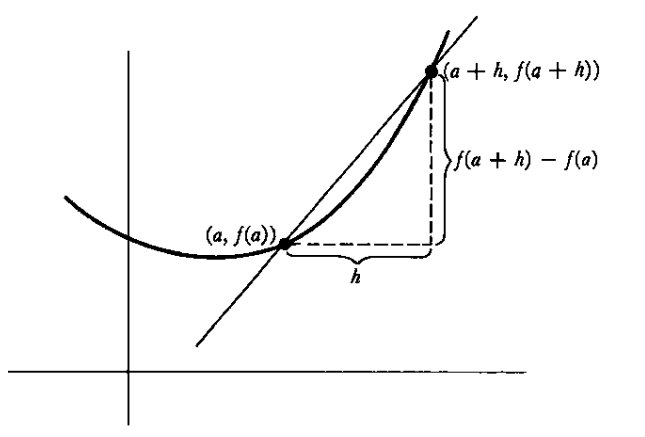
\includegraphics[width=.8\textwidth]{derivative.png}
    \caption{Geometrically, the derivative of a real function at a point $x_0$ is the tangent line at $x_0$.
    Figure taken from \cite{spivak}.}
\end{figure}

\section{Increasing and decreasing functions. Critical points}
%Derivatives give us a lot of information about how a function behaves.

\begin{defi}
    Let $\appl{f}{\R}{\R}$, then $f$ is said to be
    \begin{itemize}[itemsep = -2pt]
        \item \textbf{increasing} in $I\subseteq\R$ if $x\leq y\implies f\left( x \right) \leq f\left( y \right) $ for all $x, y\in I$, or equivallenty, if the difference quotient is non-negative,
            \begin{equation}
                \frac{f\left( y \right) - f\left( x \right) }{y - x} \geq 0,\quad\forall\ x, y\in I.
            \end{equation}
        \item \textbf{decreasing} in $I\subseteq\R$ if $x\leq y\implies f\left( x \right) \geq f\left( y \right) $ for every $x, y\in I$, or equivallenty, if the difference quotient is non-positive,
            \begin{equation}
                \frac{f\left( y \right) - f\left( x \right) }{y - x} \leq 0,\quad\forall\ x, y\in I.
            \end{equation}
    \end{itemize}
\end{defi}

\begin{lemma}\label{lem:monotony-lemma}
    Let $\appl{f}{\R}{\R}$ a differentiable function in an interval $I\subseteq\R$. Then $f$ is
    \begin{itemize}[itemsep = -2pt]
        \item \textbf{increasing} in $I\subseteq\R\iff f'\left( x \right) \geq 0$, $\forall\ x\in I$.
            \item \textbf{decreasing} in $I\subseteq\R\iff f'\left( x \right) \leq 0$, $\forall\ x\in I$.
    \end{itemize}
\end{lemma}

\begin{defi}
    Let $\appl{f}{\R}{\R}$. Then,
    \begin{itemize}[itemsep = -2pt]
        \item $\overline{x}$ is a maximum for $f$ in $I\subseteq\R$, if $f\left( x \right) \leq f\left( \overline{x} \right)$ for every $x\in I$, and it is written as $f\left( \overline{x} \right) = \underset{x\in I}{\max}f\left( x \right) $.
        \item $\underline{x}$ is a minimum for $f$ in $I\subseteq\R$, if $f\left( x \right) \geq f\left( \underline{x} \right)$ for every $x\in I$, and it is written as $f\left( \underline{x} \right) = \underset{x\in I}{\min}f\left( x \right) $.
    \end{itemize}
\end{defi}

\begin{defi}[Critical point]
    A critical point of a function $f$ is a number $x$ such that $f'\left( x \right) = 0$. The number $f\left( x \right) $ is called a \textbf{critical value} of $f$.
\end{defi}

\begin{lemma}\label{lem:critical-points-max-min}
    Let $\appl{f}{\R}{\R}$ be a differentiable function in $I\in\R$. Then, the maximum and minimum in $I$ are
    critical points. In general, the converse is not true.
\end{lemma}

Looking for the extremes of a functions, one should look in the critical points, but only in points where the
function is not differentiable and in the extremes of the domain of the function.


\hide{
\begin{theorem}
    Let $f$ be a function defined on $\left( a, b \right) $. If $x$ is a maximum (or a minimum) point for $f$
    on $\left( a, b \right) $, and $f$ is differentiable at $x$, then $f'\left( x \right) = 0$.
\end{theorem}

\begin{proof}
    Consider that $f$ has a maximum at $x$. If $h$ is a number such that $x + h\in\left( a, b \right) $, then
    $f\left( x \right) \geq f\left( x + h \right) $, since $f$ has a maximum on $\left( a, b \right) $ at $x$.
    This means that $f\left( x + h \right) - f\left( x \right) \leq 0$. Thus, if $h > 0$ we have
    \begin{equation}
        \frac{f\left( x + h \right) - f\left( x \right) }{h} \leq 0 \implies \lim_{h\to 0^+} \frac{f\left( x + h \right) - f\left( x \right) }{h} \leq 0.
    \end{equation}
    On the other hand, if $h < 0$, we have
    \begin{equation}
        \frac{f\left( x + h \right) - f\left( x \right) }{h} \geq 0 \implies \lim_{h\to 0^-} \frac{f\left( x + h \right) - f\left( x \right) }{h} \geq 0.
    \end{equation}
    By hypothesis, $f$ is differentiable at $x$, so these two limits must be equal, in this case, to $f'\left( x \right) $. This means that $f'\left( x \right) \leq 0$ and $f'\left( x \right) \geq 0$, from which follows
    that $f'\left( x \right) = 0$.
\end{proof}

\noindent The converse of this theorem is not true.
}

\begin{theorem}
    Suppose $f'\left( x \right) = 0$. If $f''\left( x \right) > 0$, then the function $f$ has a local minimum
    at $x$; if $f''\left( x \right) < 0$, then $f$ has a local maximum at $x$.
\end{theorem}

\begin{proof}
    Let $x = x_0$. By definition,
    \begin{equation}\label{eq:extremals-thm-proof-1}
        f''\left( x_0 \right) = \lim_{h\to 0}\frac{f'\left( x_0 + h \right) - f'\left( x_0 \right) }{h}.
    \end{equation}
    Since $f'\left( x_0 \right) = 0$, (\ref{eq:extremals-thm-proof-1}) can be written as
    \begin{equation}
        f''\left( x_0 \right) = \lim_{h\to 0}\frac{f'\left( x_0 + h \right) }{h}.
    \end{equation}
    Suppose now that $f''\left( x_0 \right) > 0$, then $f'\left( x_0 + h \right) / h$ must be positive for a
    small $h$. Therefore, $f'\left( x_0 + h \right)$ must be positive for a sufficiently small $h > 0$ and
    $f'\left( x_0 + h \right) / h$ must be negative for a sufficiently small $h < 0$. By \eref{lem:monotony-lemma}, $f$ is increasing in some interval to the right of $x_0$ and it is decresing in some interval to the
    left of $x_0$. Consequently, $f$ has a local minimum at $x_0$.

    \noindent The proof for the case $f''\left( x_0 \right) < 0$ is analogous.
\end{proof}

\hide{
\section{Convexity and concavity}
\begin{defi}
    A function $f$ is convex on an interval if for $a$, $x$ and $b$ in the interval with $a < x < b$ we have
    \begin{equation}
        \frac{f\left( x \right) - f\left( a \right) }{x - a} < \frac{f\left( b \right) - f\left( a \right) }{b - a}.
    \end{equation}
    In the same way, a function $f$ is concave if
    \begin{equation}
        \frac{f\left( x \right) - f\left( a \right) }{x - a} > \frac{f\left( b \right) - f\left( a \right) }{b - a}.
    \end{equation}


    A function $f$ is convex on an interval, if for all $a$ and $b$ in the interval, the segment joining
    $\left( a, f\left( a \right)  \right) $ and $\left( b, f\left( b \right)  \right) $ lies above the
    graph of $f$.
\end{defi}
}

\section{Mean Value theorems}
\begin{theorem}[Rolle's theorem]\label{thm:rolle}
    Let $f\in C^0\left( [a, b] \right) \cap C^1\left(\left( a, b \right)\right) $ such that $f\left( a \right)  = f\left( b \right) $. Then, there exists a critical point in $\left( a, b \right) $, in other words,
    there exists $c\in \left( a, b \right) $ such that $f'\left( c \right) = 0$.
\end{theorem}

This is an example of a reference to \nref{thm:rolle}.

\begin{proof}
    Since $f$ is continuous on $[a, b]$, it has a maximum and a minimum value on $[a, b]$. Suppose that the
    maximum value takes place at a point $x\in\left( a, b \right) $. Then, by \eref{lem:critical-points-max-min}, $f'\left( x \right) = 0$, and we are done.

    \noindent Suppose now that the minimum value of $f$ ocurrs in $x\in\left( a, b \right)$. Then, again
    by \eref{lem:critical-points-max-min}, $f'\left( x \right) = 0$.

    \noindent Finally, suppose that the maximum and minimum values both occur at the end points. Since $f\left( a \right) = f\left( b \right) $, both points are equal, so $f$ must be a constant function, and therefore we
    could choose any $x\in\left( a, b \right) $.
\end{proof}

\begin{theorem}[Cauchy's mean value theorem]\label{thm:mv-cauchy}
    Let $f, g\in C^0\left( [a, b] \right) \cap C^1\left( \left( a, b \right) \right) $. Then, there exists
    a point $c\in\left( a, b \right) $ such that
    \begin{equation}
        \left( f\left( b \right) - f\left( a \right)  \right)g'\left( c \right) = \left( g\left( b \right) - g\left( a \right)  \right) f'\left( c \right),
    \end{equation}
    and if $g\left( a \right) \neq g\left( b \right)$ and $g'\left( c \right) \neq 0$ we have
    \begin{equation}
        \frac{f'\left( c \right) }{g'\left( c \right) } = \frac{f\left( b \right) - f\left( a \right) }{g\left( b \right) - g\left( a \right) }.
    \end{equation}
    Here, the point $c$ of both $f$ and $g$ is the called the \textbf{mean value}.
\end{theorem}

\hide{
\begin{proof}
    Let
    \begin{equation}
        h\left( x \right) = f\left( x \right) - \brackets{\frac{f\left( b \right) - f\left( a \right) }{b - a}}\left( x - a \right).
    \end{equation}

\end{proof}
}

\begin{theorem}[Lagrange's mean value theorem]\label{thm:mv-lagrange}
    Let $f\in C^0\left( [a, b] \right) \cap C^1\left( \left( a, b \right)  \right) $. Then, there exists a
    point $c\in\left( a, b \right) $ such that
    \begin{equation}
        f\left( b \right) - f\left( a \right) = f'\left( c \right) \left( b - a \right).
    \end{equation}
\end{theorem}

These three theorems, known as the \textit{mean value theorems} for differentiation, are equivalent. Rolle's
theorem is just a special case of Cauchy's when $f\left( a \right) = f\left( b \right) $. In the same way,
if $g\left( x \right) = x$ for all $x$, then $g'\left( x \right) = 1$, and we obtain Lagrange's mean value theorem.

The mean value theorems are specially useful for proving inequalities. Take for instance $e^x\geq 1 + x$, $\forall x\in\R$. Using Lagrange's theorem in the open interval $\left( 0, x \right) $, we get that there exists
$c\in\left( 0, x \right) \geq 0$. Then,
\begin{equation}
    e^x - e^0 = e^c\left( x - 0 \right) = e^cx \geq x\quad\implies\quad e^x - 1\geq x\quad\implies\quad e^x\geq 1 + x.\qed
\end{equation}

\begin{theorem}[L'Hôpital's rule]
    Let $f, g\in C^0\left( [a, b] \right) \cap C^1\left(\left( a, b \right)\right) $ and let $c\in\left( a, b \right) $ such that $f\left( c \right) = g\left( c \right) = 0$ and $g'\left( x \right) \neq 0$ if $x\neq c$.
    If the limit $L\in\R$ of $f'\left( x \right)  / g'\left( x \right) $ exists when $x\to c$, then the
    limit of $f\left( x \right) / g\left( x \right) $ on $c$ exists and it is equal to $L$. Therefore,
    \begin{equation}
        \lim_{x\to c}\frac{f\left( x \right) }{g\left( x \right) } = \lim_{x\to c}\frac{f'\left( x \right) }{g'\left( x \right) }.
    \end{equation}
\end{theorem}

\section{Taylor's expansion}
\subsection{Higher-order derivatives}
If a function $f\in C^1\left( I \right) $ has a derivative $f'\in C^1\left( I \right) $, in other words, if
$f'$ is differentiable on $I$, then $f$ is said to be 2-times differentiable, $f\in C^2\left( I \right) $,
and the derivative is written as
\begin{equation}
    \dv{2}{f}{x}\left( x \right) = f''\left( x \right) = f^{\left( 2 \right) }\left( x \right).
\end{equation}
The same applies for $n$-derivatives. If $f\in C^n\left( I \right) $, the order $n$ derivative is written as
\begin{equation}
    \dv{n}{f}{x}\left( x \right) = f^{\left( n \right) }\left( x \right).
\end{equation}

\hide{
For any function $f$ we can obtain, by taking the derivative, a new function $f'$. The notion of differentiability can also be applied to the function $f'$, yielding another function $\left( f' \right)'$, whose domain
consists of all points $x_0$ such that $f'$ is differentiable at $x_0$. The function $\left( f' \right)' =
f''$ is called the \textit{second derivative} of $f$. If $f''\left( x_0 \right) $ exists, then $f$ is said to
be 2-times differentiable at $x_0$.

\noindent The various functions $f^{\left( n \right) }$, for $n\geq 2$, are called \textit{higher-order derivatives} of $f$.
}

\begin{defi}[Generalized Leibniz's rule]
    \begin{equation}
        \left( fg \right)\left( x \right) = \sum_{k=0}^n\comb{n}{k} f^{\left( n - k \right) }\left( x \right) g^{\left( k \right) }\left( x \right).
    \end{equation}
\end{defi}

\subsection{Infinitesimals and Landau symbols}
Let $\appl{f, g}{I\subseteq\R}{\R}$ and $x_0\in I$ such that $\lim_{x\to x_0} f\left( x \right) \lim_{x\to x_0} g\left( x \right) = 0$. These functions are called \textbf{infinitesimals at $x_0$}. Consider the limit
\begin{equation}
    \lim_{x\to x_0}\frac{f\left( x \right) }{g\left( X \right) }= \begin{cases}
        0, \quad f = o\left( g \right), \\
        1, \quad f\sim g,\\
        L\in\R, \quad f = \mathcal{O}\left( g \right), \\
        \pm\infty,\quad g = \mathcal{o}\left( f \right).
    \end{cases}
\end{equation}

\begin{defi}[Infinitesimals]
    Let $f, g$ be two infinitesimals on $x_0$. If $f = o\left( g \right) $ ("$f$ is small-o of $g$")
    whenever $x\to x_0$, it is said that $f$ is an infinitesimal of greater order than $g$ on $x_0$. If
    $f\sim g$ whenever $x\to x_0$, it is said that $f$ is asymptote to $g$ at $x_0$. If $f = \mathcal{O}\left( g \right) $ ("$f$ is great-o of $g$") whenever $x\to x_0$, it is said that $f$ is an infinitesimal of greater
    or same order than $g$ at $x_0$.
\end{defi}

\begin{remark}
    $f = o\left( g \right) \implies f = \mathcal{O}\left( g \right) $ when $L = 0$.
\end{remark}


\begin{defi}[Contact order]
    Let $\appl{f, g}{I\subseteq\R}{\R}$. It is said that $f$ and $g$ have a contact of order greater than $k$
    at the point $x_0$ if $f\left( x \right) - g\left( x \right) = o\left( \left( x - x_0 \right)^k \right) $.
\end{defi}

\begin{theorem}
    Let $f, g$ be functions $k$-times differentiable at $x_0\in I$. Then $f$ and $g$ have contact of order $k$
    at $x_0 \iff$ all the derivatives coincide at $x_0$, in other words,
    \begin{equation}
        f\left( x \right) - g\left( x \right) = o\left( \left( x - x_0 \right)^k \right)\quad \iff\quad
        f^\left( n \right) \left( x_0 \right) = g^\left( n \right) \left( x_0 \right),\quad \forall\ n = 0, \ldots, k.
    \end{equation}
\end{theorem}

\begin{theorem}[Taylor's polynomial]
    Let $\appl{f}{I}{\R}$ be a function $k$-times differentiable at $x_0\in I$. The Taylor's polynomial of
    order $k$ of $f$ at $x_0$ is given by
    \begin{equation}
        T_kf\left( x, x_0 \right) = \sum_{n=0}^k\frac{f^{\left( n \right) }\left( x_0 \right) }{n!}\left( x - x_0 \right)^n.
    \end{equation}
    Then, $T_kf\left( x, x_0 \right) $ has contact with $f$ of order equal or greater than $k$ at $x_0$,
    \begin{equation}
        f\left( x \right) = T_kf\left( x, x_0 \right) + o\left( \left( x - x_0 \right) ^k \right) = T_kf\left( x, x_0 \right) + R_k\left( x, x_0 \right).
    \end{equation}
    The last term is called Peano's remainder and it is of the form
    \begin{equation}
        R_k\left( x, x_0 \right) = o\left( \left( x - x_0 \right) ^k \right) = h\left( x \right)\left( x - x_0 \right), \quad \lim_{x\to x_0}h\left( x \right) = 0.
    \end{equation}
\end{theorem}
